%!TEX root = thesis.tex
\chapter{Method}
\label{chapter:Method}

\textbf{Introduce Method chapter}

\section{Data Collection} % (fold)
\label{sec:data_collection}

\subsection{Types of Evolution Data} % (fold)
\label{sub:types_of_evolution_data}

There are broadly 3 categories of data we could conceivably use for software evolution studies:

\begin{table*}[t]
\centering
\begin{tabular}{|p{.23\textwidth}|p{.72\textwidth}|}
\hline
{\bf History} & {\bf Description}\\
\hline \hline
Release History & Source code, binaries, release notes, and release documentation\\
\hline
Revision History & Version control logs, issue/defect records, Modification history of documentation, Wiki logs\\
\hline
Project History & Messages (email, Instant message logs), Project documentation (plans, methodology, process)\\
\hline
\end{tabular}
\vspace{0.2cm}
\caption{The different types of histories that typically provide input data for studies into software evolution.}
\label{tab:Histories}
\vspace{-0.2cm}
\end{table*}

\textbf{Cover what type of studies the different types of histories are appropriate}

\textbf{Say that we're using release-history for our study and outline some other studies that have used it to some success...include those directly studying vocabulary/vocabulary evolution}

\textbf{Provide a justification as to why we have chosen release-based history for the purposes of our study -- include our rationale (i.e. what it enables us to do/find out)}

% subsection types_of_evolution_data (end)

\subsection{Open Source Software (OSS)} % (fold)
\label{sub:open_source_software_oss_}

\textbf{Outline that we will be using OSS for our studies}

\textbf{Briefly cover why we've chosen OSS for our studies, as opposed to commercial projects}

\textbf{Highlight the benefits of using OSS}

\textbf{Rationalise that we are not missing anything too vital by not using commercial projects for our study}

% subsection open_source_software_oss_ (end)

\subsection{Open Source Project Repositories} % (fold)
\label{sub:open_source_project_repositories}

\textbf{List the places we got our systems from}

% subsection open_source_project_repositories (end)

\subsection{Selection Criteria} % (fold)
\label{sub:selection_criteria}

\textbf{List the selection criteria that we've used and descriptions for each}

\subsubsection{Rationale of Selection Criteria} % (fold)
\label{ssub:rationale_of_selection_criteria}

\textbf{TODO: Few sentences for each criterion -- can probably cite Raj's work here for bolstering rationale}

% subsubsection rationale_of_selection_criteria (end)

% subsection selection_criteria (end)

\subsection{Selected Systems} % (fold)
\label{sub:selected_systems}

\textbf{Outline the categorisation scheme chosen for our studies}

\textbf{Briefly cover the systems selected and any noteworthy information}

\textbf{Table of systems selected for analysis}

% subsection selected_systems (end)

% section data_collection (end)

% Note: This section might need to come a bit later
\section{Statistical Measures} % (fold)
\label{sec:statistical_measures}

% Sub - Identify metrics we will be using (Should probably cover what RSN is, as in Raj's thesis)
% 
% - Gini
% - Gini box plots!
% - Frequency Distribution
% - Spearman?

% section statistical_measures (end)

\section{Research Questions} % (fold)
\label{sec:research_questions}

\textbf{What are the growth patterns exhibited by vocabulary in source code?}

\textbf{How are terms distributed?}

\textbf{Does vocabulary follow laws of software evolution}

% section research_questions (end)

\section{Version Extraction} % (fold)
\label{sec:version_extraction}

\textbf{Introduce section by covering what information we need to extract for our study}

\textbf{Cover, broadly, how we intend to obtain this information from the choice of data we opted for}

\textbf{Introduce Mutations as being the tool to solve all of our woes}

\textbf{Broadly cover what Mutations does and what it is capable of}

Mutations works by utilising the ASM bytecode manipulation framework to extract various properties from binary Java class (.class) files. Such properties include x, y and z. The tool, by default, also extracts the names of each of the fields, methods, interfaces and other such information associated with a class. All of this information is stored as JSON formatted data in plain-text files.

\textbf{Detail how Mutations goes about extracting the information from input JAR files}

\textbf{Cover in some depth, each stage Mutations goes through to obtain the data}

% section version_extraction (end)

\section{Vocabulary Definition} % (fold)
\label{sec:vocabulary_definition}

\textbf{Justify the definition of a vocabulary (i.e. why do we need to be precise about vocabulary? Need a consistent representation for comparison!)}

\textbf{Cover the definitions of others, what they lacked and what we have drawn upon from them.}

\textbf{Cover what we need from a definition (might want to shift this above previous paragraph). i.e. What do natural language vocabularies have relating to mental models that needs to be captured in programmer language.}

\textbf{Explain (at a high-level) our approach to defining vocabulary for our study, in light of the constraints outlined in previous paragraphs. (i.e. we wanted a representation of vocabulary that was quasi-unique to individual system -- containing only terms that are likely to be the cause of cognitive overload)}

\textbf{We defined vocabulary as being being composed of the complete set of class names, method names and field names accumulated from each class within a given release of a software system.}

\textbf{The use of compound identifiers within software systems is common. While the compounding of words is often used to merge together to concepts within a given context, e.g. or even take on new meanings altogether TODO: Example of these. (can list this as a limitation...in general, our vocabulary definition has glaring holes). We made the assumption that terms compounded together within programmer language adhere to the former, and thus, selected to treat each single word within the language as a distinct element of the vocabulary.}

\textbf{TODO: Be more specific about terminology -- identifiers, words, tokens, terms, lexicon}

% section vocabulary_definition (end)

\section{Vocabulary Extraction} % (fold)
\label{sec:vocabulary_extraction}

The class metric data extracted for each version of the systems used for our analysis provides the basis for forming the representation of vocabulary.

In order to build our vocabulary, we need terms. The vocabulary that we will use will be composed of various linguistic elements of the source code, including the following:

\begin{enumerate}
	\item Class names
	\item Method names
	\item Field names
\end{enumerate}

From these elements, we extract individual words. Precise/consistent extraction of distinct keywords from compound identifiers is a non-trivial task (even understanding these keywords can be difficult). \textbf{TODO: Need examples of coding styles or lack thereof producing hard to understand}. The use of adopted and well-adhered to coding standards aids in presenting identifiers in a clear and consistent manner. The coding standard for Java which has been prescribed by Sun \textbf{TODO: Is this in fact Sun's coding standard? Can we cite it?} \textbf{TODO: A compare and contrast example of using the Java coding standard and not using it} (and adapted by many projects) is conformed to by a number of open-source projects.
In addition to this, there are popular tools which integrate into the build process which allow projects to enforce the use of such standards.

\textbf{Note: the above points add weight to the notion that splitting based on the Java coding standard is somewhat sufficient -- lots of projects use it + there are tools that are capable of enforcing it -- we basically want to sell that it is adhered to well enough that we can use it as a basis for splitting identifiers into appropriate words}

\textbf{TODO: Might want to sneak this in here...or in limitations}
Need more sophisticated means of extracting distinct terms from identifiers to build a more representative vocabulary.

Because of this, we use the Java coding standard as the basis for separating identifiers into individual elements of the vocabulary.

\textbf{Outline the standards for the elements we will be extracting terms from and what they would yield -- examples}

\begin{itemize}
	\item Camel case
	\item Pascal case
	\item Upper-case and underscore separated
\end{itemize}

Report|Writer
report|Writer
REPORTWRITER

\textbf{Outline how we actually go about extracting the terms from the data we have}

\textbf{Extraction process diagram}
JAR Extractor -> Class Metric Extraction -> Class Vocabulary Extraction -> Class Vocabulary Merging -> Vocabulary Metric Extraction

For building our representation of vocabulary for the systems we analysed, we extended the capabilities of an existing software evolution analysis tool, \emph{Mutations}.

Using Mutations, we get programmatic access to this information through the ClassMetricData abstraction, which encapsulates the metadata associated with classes highlighted in the previous paragraph.

First, we use Mutations to extract the class metric data, as described in Section \textbf{TODO: Refer to section here}. Once we have extracted each class in the version, we begin to extract the vocabulary from each of the ClassMetricData objects. This entails the mining of words from the set of both method names and field names for each class within the version. In order to keep track of our vocabulary whilst processing the sets of identifiers, we maintain a map of class name -> token -> occurrences (i.e. the number of times a token has been used). With each occurrence within an identifier, we increment the occurrence count for the token encountered.

\begin{figure}[t]
	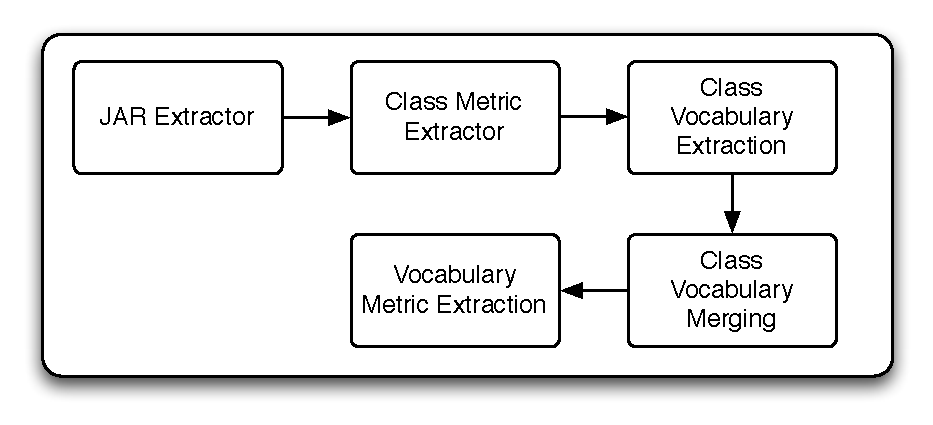
\includegraphics[width=\textwidth]{VocabMetricExtraction.pdf}
	\caption{Vocbulary metric extraction process.}
	\label{fig:VocabMetricExtraction}
\end{figure}

\textbf{TODO: Need trim list justification/description somewhere above}

\textbf{TODO: Borrow from Raj's thesis for a description of what Mutations does}

\textbf{Token extraction algorithm for different elements -- include reg-ex}

\begin{lstlisting}[caption={Same of bytecode generated for a simple Hello World method}, label={BytecodeExample}, float=t]
	/** **/
	public void extractVocabulary(History history)
	{
		for(Version version : history.getVersions())
		{
			for(ClassMetricData classMetricData : version.getVersions())
			{
				extractClassNameTokens(classMetricData.getClassName());
				extractMethodTokens();
				extractFieldTokens();
			}
		}
	}
	
	private void extractClassNameTokens(String className)
	{
		
	}
	
	private void extractMethodTokens(Set<String> methodSignatures)
	{
		for(String methodSignature : methodSignatures)
		{
			
		}
	}
\end{lstlisting}

\begin{table*}[t]
\centering
\begin{tabular}{|p{.40\textwidth}|p{.50\textwidth}|}
\hline
{\bf Type} & {\bf Token}\\ \hline
\multirow{9}{*}{\bf Primitives}
& class, \\
& string, \\
& char, \\
& int, \\
& long, \\
& float, \\
& double, \\
& byte, \\
& object \\
\hline
\multirow{9}{*}{\bf Unambiguous Terms}
& get, \\
& set, \\
& val, \\
& value, \\
& name, \\
& impl, \\
& listener, \\
& event, \\
& this \\
\hline
\end{tabular}
\label{tab:NotHistories}
\end{table*}

\textbf{Merging of vocabulary once the various sets have been established}

\textbf{TODO: How do we generate the measures used once we have extracted the vocabulary?}

% section vocabulary_extraction (end)